\appendix

\subsection{Relationship to other distributed systems}
\label{sec:distributed-comparison}
Blockchain technology fits within the broader family of distributed systems.
At the highest level, Blockchain technology is a type of decentralized database.
To help readers situate Blockchain technology within this greater ecosystem we have created a taxonomy and a flowchart based on that taxonomy (see Figure~\ref{fig:blockchainFlowchart}).

\begin{figure*}
	\centering
	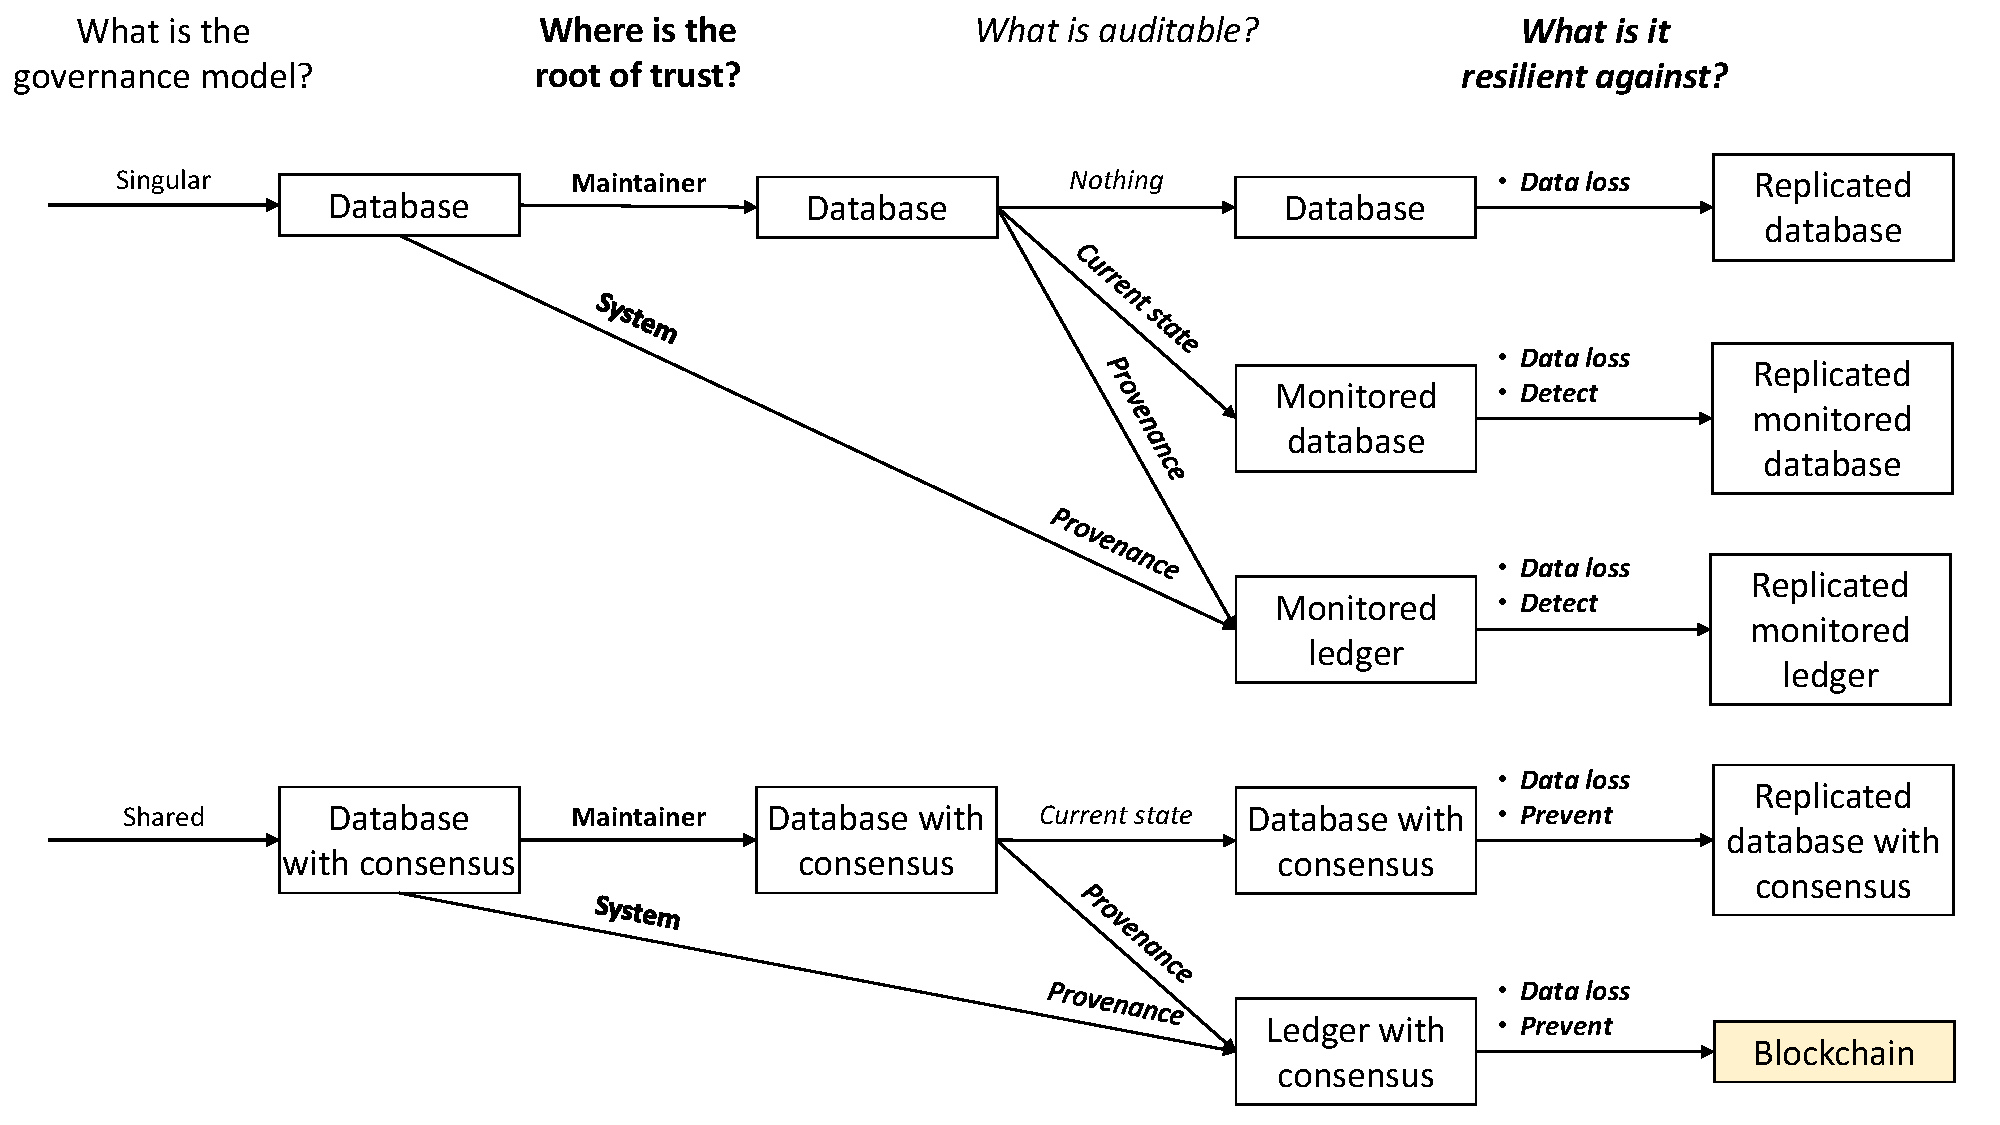
\includegraphics[width=.75\textwidth]{figures/BlockchainFlowchart}
	\caption{Comparing decentralized databases. Blockchain is highlighted in the bottom right corner.}
	\label{fig:blockchainFlowchart}
\end{figure*}

The first property in our taxonomy considers who has the authority to manage and update the database: \emph{what is the governance model?} In a centrally governed database (``Centralized''), a single entity performs these tasks. Alternatively, the system can use a consensus protocol to allow for decentralized governance (``Decentralized'').

Next, we consider the security model by asking \emph{where is the root of trust?}
This refers to the entity or entities that must behave honestly in order for the system to be secure.
In typical database systems, trust is rooted in the maintainer (``Maintainer'')---for example, using AWS cloud storage requires that you trust Amazon.
Alternatively, trust can be rooted in the design of the system itself (``System''), though this is only possible if the system stores sufficient provenance for it to be audited to confirm that the system is functioning as intended.

The next question is \emph{what is auditable?}
In the worst case, nothing is auditable (``Nothing'').
Systems can use an authenticated data structure~\cite{tamassia2003authenticated} to ensure that their current state can be audited (``Current state'').
If the state also contains a history of the system (e.g., a ledger), then the use of an authenticated data structure allows for the provenance of the system to also be audited (``Provenance'').
In both cases, it is necessary that these databases be monitored to ensure that they never enter an invalid state, even temporarily.
In the case of decentralized systems, the decentralized partners can act as monitors.

Finally, we can classify systems by asking \emph{what is it resilient against?}
In particular, we considered with three resiliency properties---(1) is it resilient to accidental data loss (``Data loss''), (2) is it possible to detect that data has been malicious altered (``Detect''), (3) and is it possible to prevent malicious updates (``Prevent'').
Systems with centralized governance are only able to detect malicious updates as the monitors can detect the attack but cannot prevent the malicious update from being replicated.
If we modify the system to allow monitors to play this role, they have become consensus partners and we now have a decentralized database.

\subsection{Survey of Academic Research on Challenges}
In this section, we report on a survey we conducted that looked at research from the academic community that attempts to address challenges related to and impeding the proper and secure use of Blockchain technology.

\subsubsection{Power consumption and centralization of mining}
To reduce the power consumption of Blockchain, there have been several proposals to turn to other consensus mechanisms that do not rely on proof of work.  The most popular of these proposals is proof of stake consensus, where parties' contribution to the consensus protocol is proportional to the total amount of stake they own in the system rather than the amount of work that they do.  This allows consensus to be achieved without relying on wasteful proofs of work.  Today's proof of stake protocols (e.g.~\cite{FC:BenGabMiz16,eprint:BenPasShi16,CRYPTO:KRDO17,SOSP:GHMVZ17}) vary significantly in their model, assumptions, and performance guarantees.  Other suggestions for avoiding proofs of work include proof of space~\cite{CRYPTO:DFKP15, eprint:PPKAFG15} where miners use storage instead of computation, and proof of elapsed time~\cite{SSS:CXSGLS17} where trusted hardware (i.e., Intel SGX) is used in place of proofs of work.  It is not clear at this point which solution will be best suited for different blockchain deployments.  

One possible solution~\cite{CCS:MKKS15} is to discourage mining pool formation by making it impossible to enforce cooperation between the members.

\subsubsection{Increasing transaction rates}
Another challenge to the scalability of Blockchain solutions, especially in the permissionless setting, is the increasing number of transactions.
Current systems often have rather long wait times before a transaction can be confirmed on the blockchain (e.g., Bitcoin can take several hours to confirm a transaction~\cite{BlockchainInfoTransactionConfTime}).  This makes blockchain-based solutions less than ideal when immediate transactions are needed, such as when purchasing physical goods.

A couple of different approaches have been proposed to deal with this issue.  First, a number of hybrid consensus algorithms (e.g.,~\cite{SOSP:GHMVZ17,OPODIS:AMNRS17,DISC:PasShi17,EC:PasShi18,NSDI:EGSR16}) aim to reduce transaction approval times through reducing or eliminating forks. Most of these work by using ``proof-of'' style protocols to elect a committee or a leader who then uses traditional byzantine fault-tolerant consensus to advance the blockchain.  A second approach for improving transaction rates, especially for financial transactions, is to make use of payment-channel networks. Such networks set up pairwise channels between parties to allow transactions on these channels to occur ``off-chain'', i.e., without being recorded on the blockchain; the blockchain is only used for conflict resolution.  Many different flavors of payment-channel networks achieving various properties have been proposed (e.g.~\cite{PooDry16, NDSS:HABSG17,CCS:KhaGer17,SYSTOR:LNEKPS18,CCS:MMKMR17,CCS:GreMie17}) and several such as the Lightning network~\cite{PooDry16} are in active development for financial transactions on top of Bitcoin.  

\subsubsection{Handling increased transaction volume}
Another scalability challenge for popular blockchain-based systems such as Bitcoin and Ethereum is the sheer volume of transactions that are being added to the blockchain.  As more and more third-party services start to use these blockchains to store and execute their transactions, these systems have to verify and store transactions for a variety of unrelated operations. This can cause the storage and verification work required of miners to become prohibitively expensive.

Proposed solutions for this problem include sharding (e.g.~\cite{CCS:LNZBGS16, FC:GenRenSir17}) to partition transactions based on the transaction type or service.
This allows different sets of miners to verify transactions for different services thus reducing the amount of verification work each miner must do.  Another more radical approach to deal with this challenge has been to move away from the ``chain'' view of blockchain.  Instead, several proposals (e.g., ~\cite{ePrint:SomLewZoh16,eprint:SomZoh18,IOTA}) propose to organize transactions into a directed-acyclic graph (DAG) where later transactions can vote on the validity of earlier transactions, allowing transactions to be approved before global consensus is achieved.

As the Bitcoin user base and transaction volume have grown, limitations on its scalability have been revealed. To some degree, these limitations are a result of Bitcoin's chosen parameters; for example, the 1MB cap on block size has periodically caused prohibitively high transaction fees and wait times. This limitation was mitigated by the Bitcoin Cash hard fork in 2017, which created 8MB blocks, but other scalability problems may not be so easily solvable by simple parameter tweaking, suggesting that they may be inherent limitations of public blockchain technology. We will discuss two limitations that stem from the proof-of-work consensus model that is typically used in public blockchains: emergent centralization of control and high rates of energy consumption.

Currently, almost 70\% of Bitcoin blocks are mined by the five largest pools \cite{BlockchainInfoPools}. Of course, these pools are disincentivized to damage trust in Bitcoin (and thus reduce its value and their profits) by abusing their power to censor transactions or violate rules in other ways. But this centralization undoubtedly runs counter to the normative property that Blockchain is decentralized and may violate security notions that depend on decentralization. This problem is caused in part by the hardware-optimized Bitcoin mining puzzle, for which alternatives are being explored, but whether or not this limitation can be overcome at scale is still an open question.

Bitcoin is also an illustrative example for another inefficiency of public blockchains at scale: the energy consumption of proof-of-work consensus. According to one estimate\cite{Digiconomist}, as of April 2018 the energy consumed by Bitcoin miners is equivalent to the power usage of almost 5.5 million US households, and all signs indicate that it will continue to grow. A similar problem is likely to arise in any scheme where proof-of-work is deployed. It may be surpassable if alternative consensus protocols such as proof-of-stake are used, but there are other problems to work out with such schemes (in particular, a worsening of the emergent centralization problem discussed above). 

\subsubsection{Smart contract correctness}
Three different directions have been proposed for improving the correctness and security of smart contracts:  Education and tools to help developers write smart contracts, tools for evaluating correctness and security of existing smart contracts, and formal modeling and formal verification of smart contracts. Along the education path, researchers organized a class on developing smart contracts cataloging common mistakes and misunderstandings~\cite{FC:DAKMS16}. Additionally, tools have been developed to simplify development of \emph{private} smart contracts~\cite{SP:KMSWP16}. For evaluation of existing smart contracts, multiple tools using symbolic execution~\cite{CCS:LCOSH16}, machine learning~\cite{arxiv:Huang18}, and static analysis~\cite{CCS:BDFGGK+16,NDSS:KGDS18} have been developed for detecting bugs and vulnerabilities. Finally, some efforts to support development of formally verified smart contracts is underway; for example, the Ethereum Virtual Machine (EVM) has been fully defined for interactive theorem provers~\cite{Hirai17}, which are essential tools for building formally verified software of any kind. Magazzeni et al.~\cite{Magazzeni17} have laid out a research agenda identifying further groundwork that must be conducted to support formal verification of smart contracts.

\subsubsection{Dispute resolution and rollback of mistakes}
Despite best efforts to eliminate mistakes in smart contract and transactions, a payment or asset transfer system must be able to reverse fraudulent or errant transactions. The immutability property of Blockchain means that transactions cannot be stricken from the ledger after consensus has been reached, so alternative means of dispute resolution must be explored. A new transaction reversing the effects of the disputed transaction could be added to the ledger, but decentralized governance makes arbitrating such a dispute difficult as there is no individual arbiter with the authority to determine which party is in the right when a dispute occurs.  Additionally, dispute resolution must be handled carefully to avoid introducing new vulnerabilities.  For example, several attacks were demonstrated against the Bitcoin refund mechanism~\cite{FC:MccShaHao16} necessitating further research to design secure refunds in Bitcoin~\cite{arxiv:AviSafSha18}.

\subsubsection{Non-auditability of off-chain oracles}
Smart contracts sometimes leverage off-chain oracles: online services that provide information in response to a request. For example, gambling contracts may determine which address to pay winnings to based on the result of some oracle request (e.g., sports scores, stock prices, weather forecasts, or other global events). If contract logic branches based on the response from an off-chain oracle, that contract is no longer verifiable after the fact because auditors cannot confirm that the response received from the oracle at audit time is the same response received when the contract was executed. There are legitimate reasons why an oracle response might change with time, so this is really an inherent limitation of Blockchain technology: smart contracts cannot "see" external events.

One system tackling this problem is Town Crier~\cite{Zhang16}. It uses a trusted hardware back end (Intel SGX) to serve as an authenticated off-chain oracle for Ethereum smart contracts. This allows an auditor to later verify the oracle's response at the time at which the contract was executed. This solution sidesteps the limitation of oracle non-auditability by moving trust to a centralized location (the hardware platform providing authenticity), but it does not diffuse trust in the way our analysis reveals that Blockchain technology is expected to.

\subsection{Key Management}
Another major challenge of blockchain is that it requires users to store, manage, and secure cryptographic keys both to certify their own transactions and to verify transactions of others.  However, the challenges of maintaining and protecting such key repositories are well documented (see, e.g.~\cite{uss:WhiTyg99}).  A survey by Eskandari et al.~\cite{arxiv:ECBS18} outlines the challenges as well as potential solutions for managing keys for Bitcoin.  They discuss solutions such as password-protected and password-derived keys as well as offline and air-gapped storage of the keys.  But, as the authors state all of these solutions have their drawbacks.

Some recent work has also looked into cryptographic solutions to protect users' keys.  Techniques based on secure multi-party computation (MPC)~\cite{CCS:LinNof18,C:Lindell17} allow transactions to be signed without any party ever having access to the secret key.  Alternatively, the classic technique of threshold signatures (e.g.~\cite{PKC:Boldyreva03,EC:GJKR96,EC:Shoup00a}) allow users to split their keys into many pieces such that a large number of them must be compromised in order to ``steal'' a user's key.  However, much work remains to secure all the cryptographic keys inherent in real-world blockchain deployments.


\subsection{Technical Properties Full Diagram}

\begin{center}
	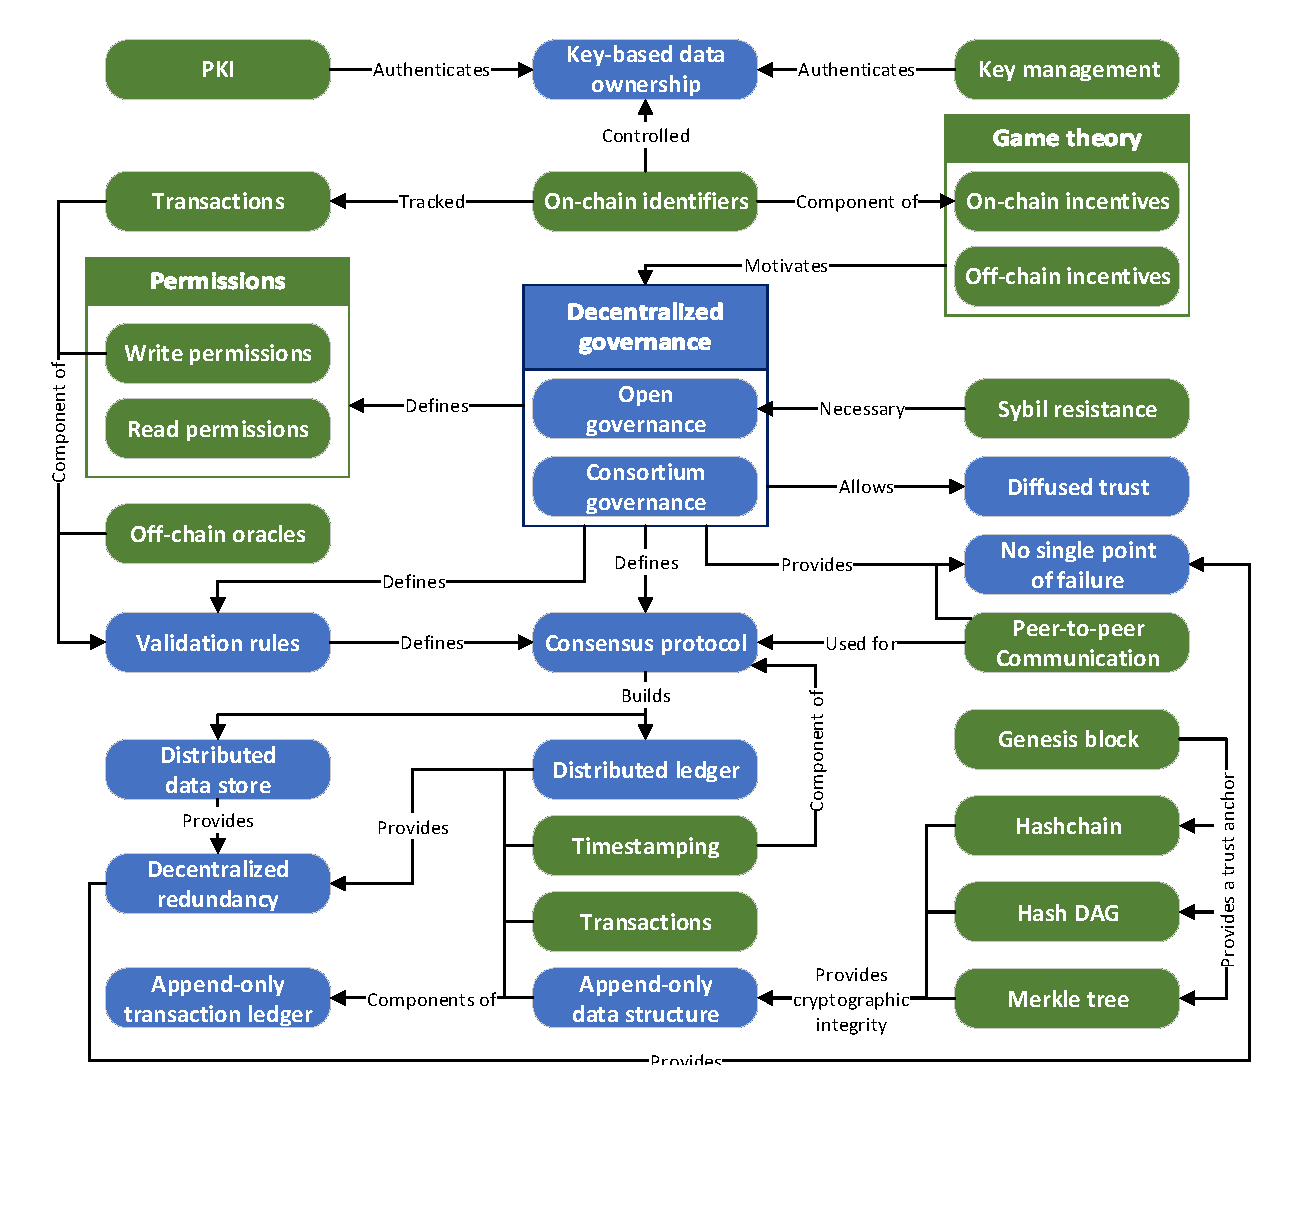
\includegraphics[page=1,width=\columnwidth]{figures/grounded-theory-main}
	\captionof{figure}{Technical Properties for Blockchain Technology With Supporting Technical Primitives}
	\label{fig:technical-properties-full}
\end{center}

%\begin{figure}
%	\centering
%	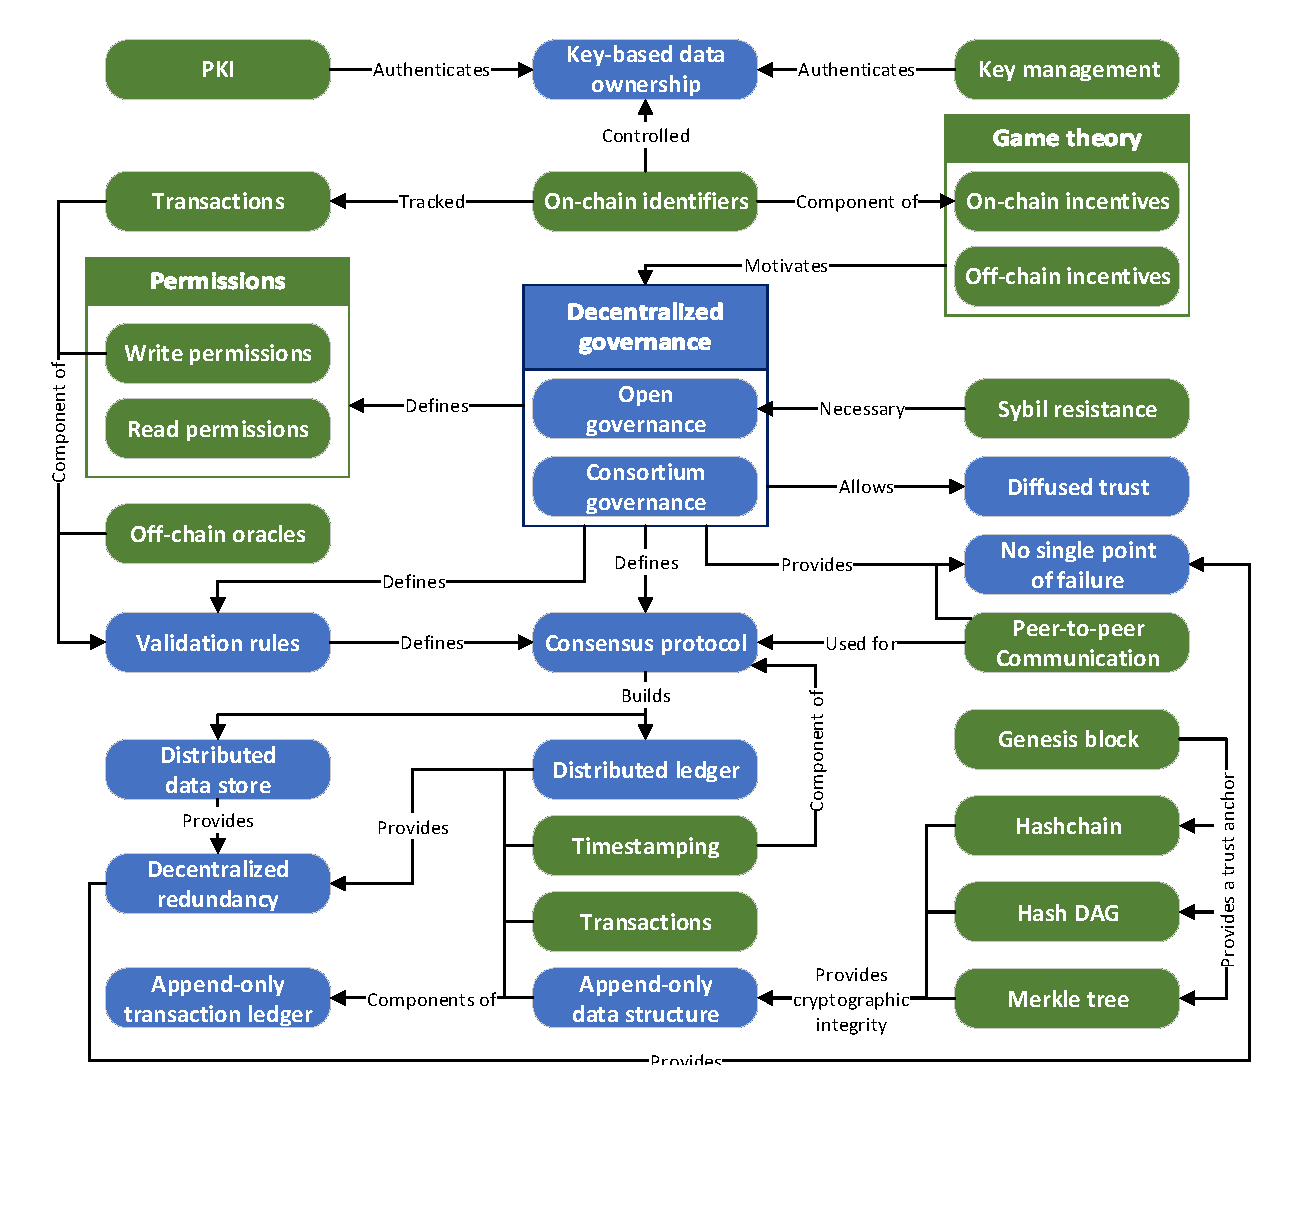
\includegraphics[page=1,width=\columnwidth]{figures/grounded-theory-main}
%	
%	Technical properties are in blue and technical primitives are in green.
%	\caption{Technical Properties for Blockchain Technology With Supporting Technical Primitives}
%	\label{fig:technical-properties-full}
%\end{figure}